\documentclass[12pt,english]{article}

\usepackage{natbib}

\usepackage{graphics,graphicx,dcolumn,bm,fleqn,epic,eepic,float}
\usepackage{amssymb,amsmath,multirow,rotate,rotating,color}
\usepackage[utf8]{inputenc}

\usepackage[english]{babel}
\usepackage{caption}
\usepackage{subcaption}
\usepackage{tikz}
\usepackage{hyperref}
\hypersetup{
    colorlinks=true,
    linkcolor=blue,
    filecolor=magenta,      
    urlcolor=cyan,
}
%\usepackage[usenames,dvipsnames,svgnames,table]{xcolor}
\tikzset{fontscale/.style = {font=\relsize{#1}}}
\usetikzlibrary{calc}
\makeatother

\newcommand{\figref}[1]{Fig.~\ref{fig:#1}}
\newcommand{\eqnref}[1]{Eq.~(\ref{eq:#1})}
\newcommand{\ts}{\textsuperscript}

\definecolor{tuered}{RGB}{214,0,74}

\newcommand{\todo}[1]{\textbf{\textcolor{tuered}{ TODO: #1}}}

\newcommand{\vectornorm}[1]{\left|\left|#1\right|\right|}

\renewcommand{\vec}[1]{\mathbf{#1}}
\newcommand{\uvec}[1]{\hat{\vec{#1}}}
\newcommand{\tensor}[1]{\mathbf{#1}}

\definecolor{pyblue}{HTML}{1F77B4}
\definecolor{pyorange}{HTML}{FF7F0C}
\definecolor{pygreen}{HTML}{2CA02C}
\definecolor{pyred}{HTML}{D62728}

\newcommand{\JH}[1]{\textcolor{blue}{JH: #1}}
\begin{document}

% The referee PDF has been generated from r239 -- 'make referee' command.


\section*{Reply to Referee B}

We thank the Referee for his/her thorough reading of our manuscript and detailed report.
We are happy to read that the referee acknowledges the amount of work we did and thinks it could be fitting for PRL after revision.
In what follows we provide detailed answers to all Referee's questions and we discuss all the changes made to the manuscript
(which are typeset in red colour).

\begin{itemize}


\item[ \textbf{\underline{Comment 1.}}]
{
The model disjoining pressure, Eq. 3 with a tail decaying as the
inverse squared power seems odd. I am more familiar with the expected
van der Waals tail with a decay as the inverse cube power. Is there
any reason for this choice?

\item[ \textbf{Answer}]
{
The Referee is right in pointing out that, indeed, the $h^{-3}$ decay 
for the attractive part of the disjoining pressure is more straightforward 
to understand as it can be derived directly from an intermolecular potential of Lennard-Jones type. Nevertheless, it is also true that other forms
can be encountered in the literature, depending on the actual interactions
\cite{PhysRevE.63.011208}. Here, though, our choice of the $(3,2)$ pair of exponents is motivated more by computational reasons rather than by the will of 
simulating a specific liquid with given physical properties.
With such choice, in fact, the characteristic dewetting time 
is shorter, thus making the overall computational cost more manageable.
In fact, we have seen in previous study~\cite{PhysRevE.104.034801} that
except for this shift of the time scales, the dewetting dynamics remains 
qualitatively the same. To confirm this observation, we have run 
a new simulation (for a single pair of pattern wavelength and speed) 
with the $(9,3)$ exponents and show the results in figure \ref{fig:rivulets_9_3}.
\begin{figure}
    \centering
    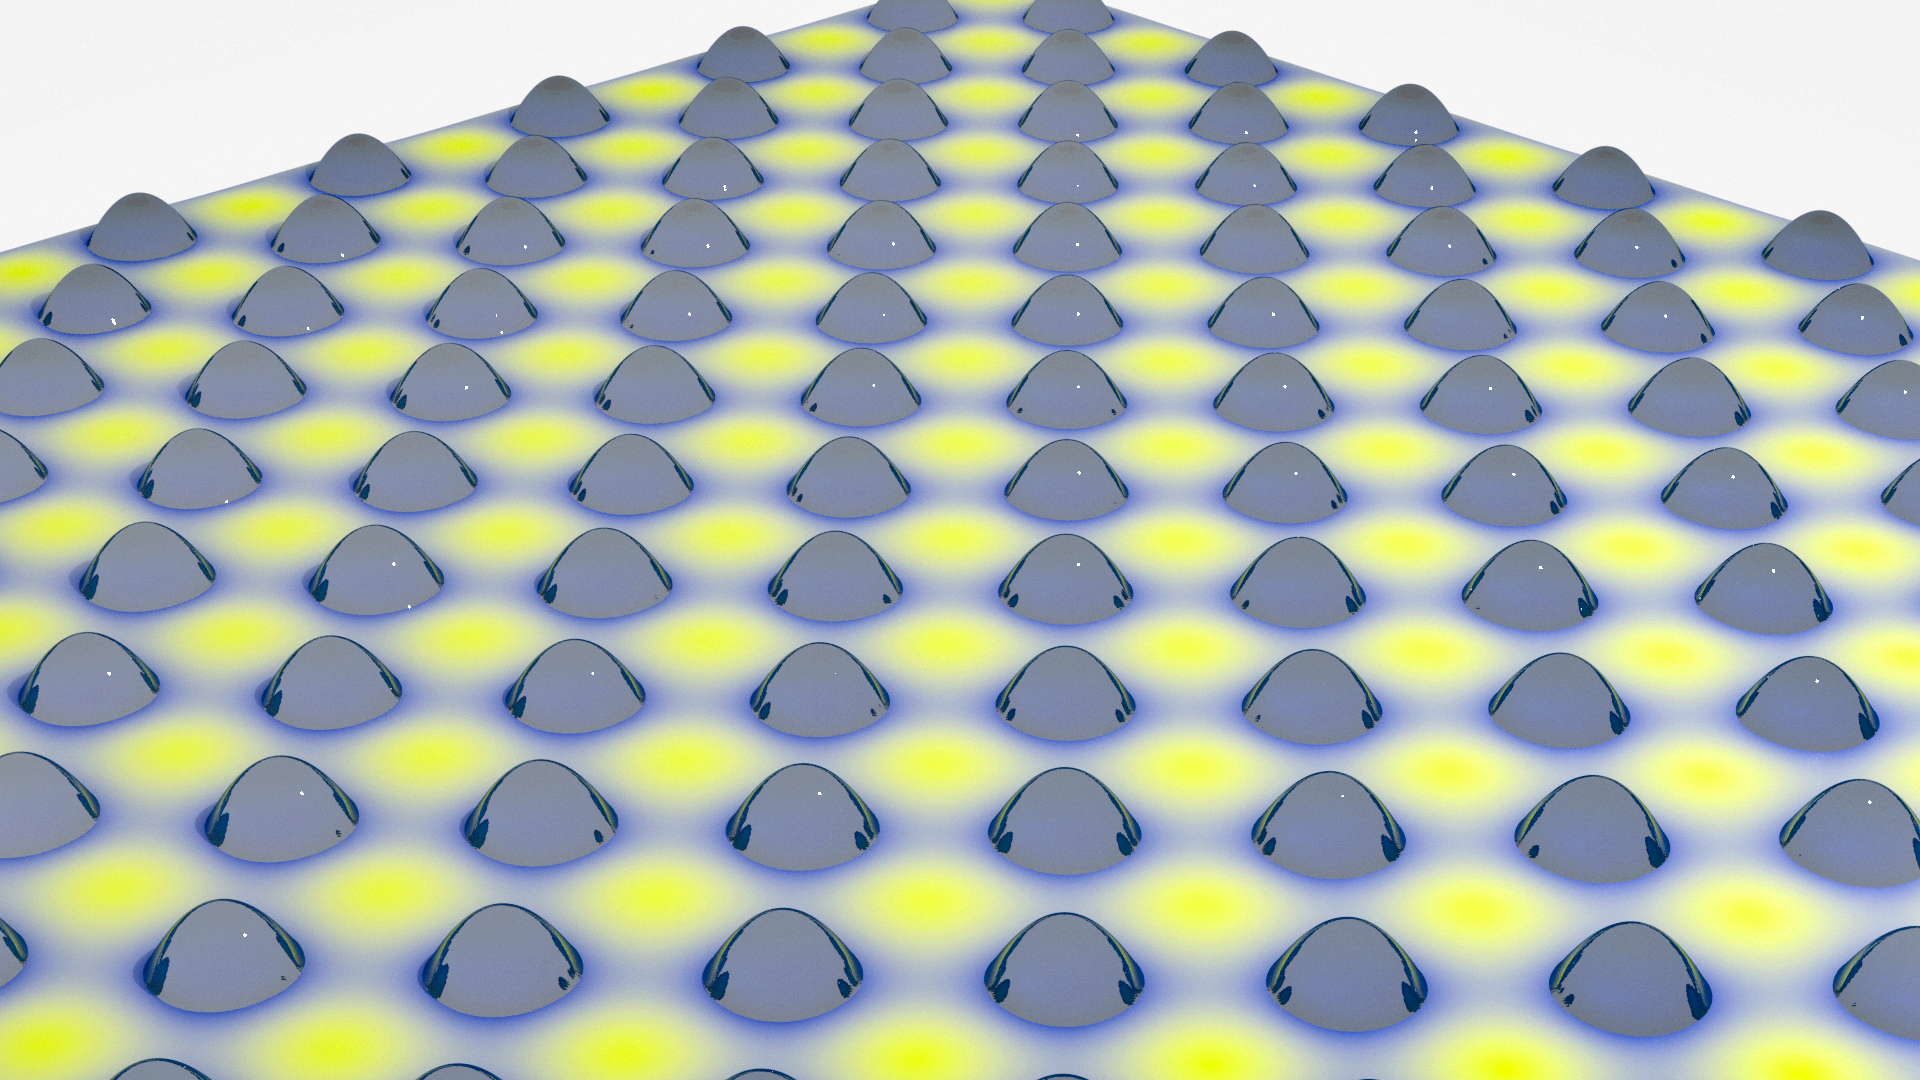
\includegraphics[width=0.45\textwidth]{Figures/No_vel_render2.png}
    \caption{}
    \label{fig:rivulets9_3}
\end{figure}
We have also added a footnote in the paper commenting on this aspect.
%We thank the referee for pointing this out.
%It is true that there are variations concerning the power law model of %the disjoining pressure.
%A common one to which the referee refers to is $(n,m) = (9,3)$, the %choice we made for the manuscript is $(n,m) = (3,2)$.
%Both exponent pairs can be found in the literature with even more %variety~\cite{moulton_lega_2013,SCHWARTZ1998173,doi:10.1063/1.4828721,Br%asjen}.
%The pair $(9,3)$ is the one that can be motivated from functional %derivatives of a Lennard-Jones potential, understandably this could more %appealing to use.
%We have used both exponent pairs in previous works, see %e.g.~\cite{PhysRevE.104.034801}.
%In this manuscript we use $(3,2)$ to keep $t_0$ reasonably small and %thus the overall computational cost manageable.
%Using the pair $(9,3)$ does not alter the results, it effectively shifts %the value of $t_0$ by $\approx 10$.
}

\item[ \textbf{\underline{Comment 2.}}]
The second major concern refers to the choice of slip length. 
The authors study a fluid-substrate model that has a thin film equilibrium thickness of 
$0.07$ length units, but the slip length is one unit, hence about $10$ times larger than the equilibrium film thickness. 
This seems unexpected, in view of the small contact angle chosen for the system. 
Could the authors justify this choice?
}

\item[ \textbf{Answer}]
{
As the Referee correctly remarks, indeed small contact angles are typically associated to small slip lengths. From a phenomenological point of view, 
though, having $\delta \sim h_0$ is still commonly considered in the weak/intermediate slip regime, as proven, for instance, 
by the formation of satellite 
droplets following rivulet breakup~\cite{doi:10.1073/pnas.1820487116} or 
in the rim shape in dewetting by hole nucleation~\cite{fetzer2007quantifying, munch2005lubrication} (see also Fig.~\ref{fig:slip}).
\begin{figure}
    \centering
    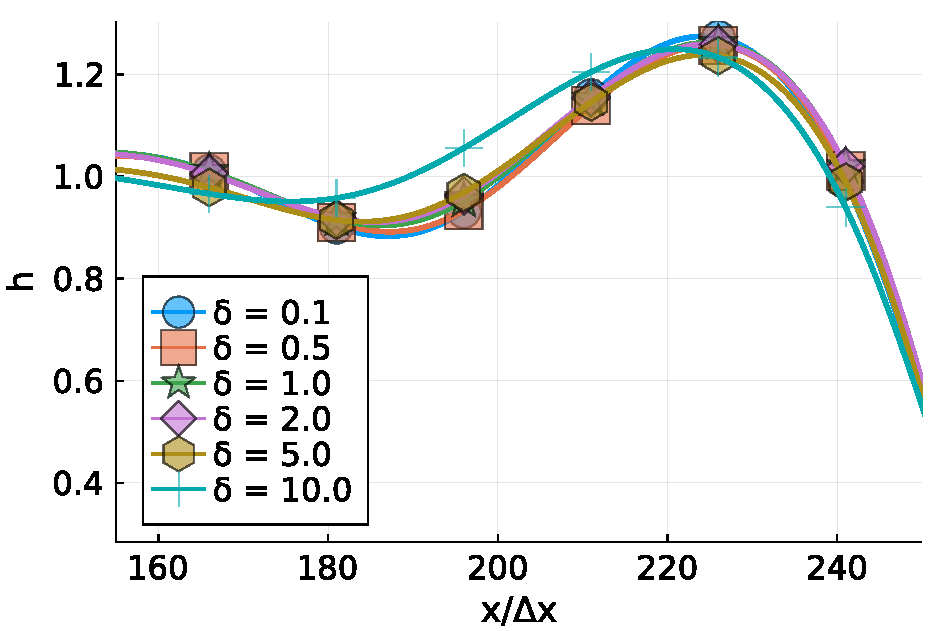
\includegraphics [width=0.6\textwidth]{slip_measure.pdf}
    \caption{Dewetting rim profiles for various slip parameters $\delta$; notice the presence of a dimple behind the front, typical of 
    small to vanishing slip, which is preserved for slip lengths up to 
    $\delta \sim 10 h_0$.}
    \label{fig:slip}
\end{figure}
Our choice of this slip length value was dictated essentially by the need 
to keep numerically stability even in the strongly time dependent case 
(large pattern speed), yet remaining in a small slip regime. 
Nevertheless, motivated by the Referee's concern and in order to check that 
picture remains qualitatively the same, we have run a simulation with 
a slip length five times smaller. The results from the analysis of the Minkowski metric $q_2$, for two cases with low and high pattern speed, reveal that indeed
the droplet-to-rivulet transition is confirmed, with $\Gamma$ as the 
discriminating parameter (see figure \ref{fig:q2smallslip}).
\begin{figure}
    \centering
    %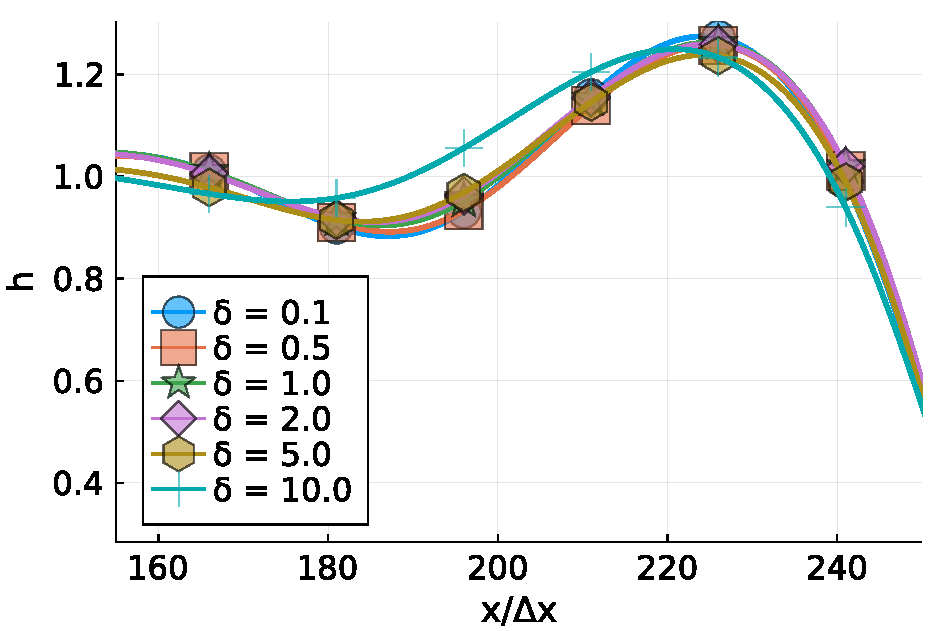
\includegraphics [width=0.6\textwidth]{slip_measure.pdf}
    \caption{}
    \label{fig:q2smallslip}
\end{figure}
We have commented on this when we give the value of the slip length, just before 
equation (5) of the revised manuscript.
%We thank the referee for bringing this up.
%Slip and disjoining pressure are an essential part of our model -- as for many %other thin film solvers.
%Here, they allow us to have moving contact lines with imposed wettability %features.
%We agree that the value may seem large at first glance.
%However, as Peschka et al. have shown, the generation of satellite droplets %during rivulet breakup, similar to what we observe, is a no-slip %feature~\cite{doi:10.1073/pnas.1820487116}.
%We observe the occurrence of satellite droplets in the initial dewetting %period.
%Increasing the slip length makes those droplets disappear.
%Another point to mention here is the dependency of the dewetting rim on the %slip.
%Small to vanishing slip induces a dimple behind the front, while for large slip %lengths this dimple vanishes~\cite{fetzer2007quantifying, %munch2005lubrication}.
%We checked this behaviour in Fig.~\ref{fig:slip} and found only a small %dependency for slip lengths $\delta < 10$.
%Spots with a thickness $h \leq h_{\ast}$ are considered dry spots, therefore %the term equilibrium thickness maybe exaturated.
}

\item[ \textbf{\underline{Comment 3.}}]
{
The relevance of the manuscript relies on the significance of the substrate's switchable properties. 
Particularly, it is assumed that the wetting properties can be modulated on space but also on time. 
The authors have mentioned in the introduction that this can be potentially done. 
However, it would be desirable that the authors relate their model of switchable substrate with some specific experimental realization, where the actual length and time scales are mentioned.
}

\item[ \textbf{{Answer}}]
{
\begin{figure}
    \centering
    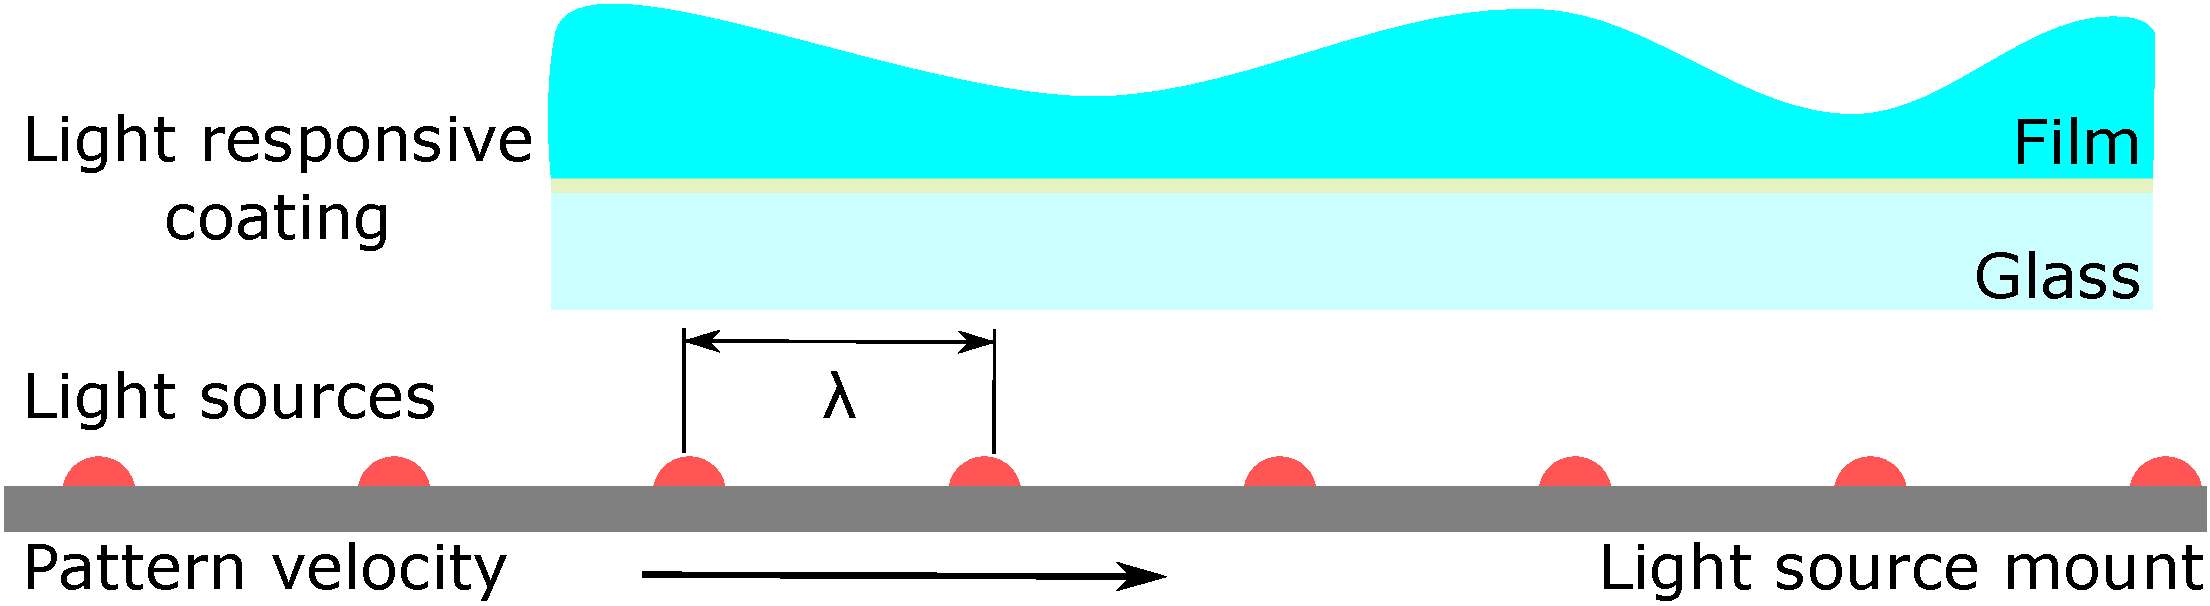
\includegraphics[width=\textwidth]{simple_exp.pdf}
    \caption{Schematic realization of the experiment described in the manuscript.}
    \label{fig:experiment_illustration}
\end{figure}
We thank the Referee for bringing this up.
First, we like to note that experiments are not our field of expertise and therefore our envisioned realization could be flawed.

The idea we have would be to prepare a thin film ($h_0 \approx 4nm$ PS) on a light responsive substrate.
Dimensions of the substrate should at least be $2$ microns in $x$ and $y$, but larger is fine.
Arrange several light sources (diodes) in a lattice with a distance of $\lambda \approx 1\mu m$ between them, as displayed in Fig.~\ref{fig:experiment_illustration}.
It would be perfect if the structure on which the light sources are mounted can be moved in a periodic manner, e.g. wrapped around rolls.
On the other hand if the array of diodes is large enough, say $100\lambda$ it should be sufficient to move them continuously in one direction. 
\JH{Could one do this with a DMD as here https://doi.org/10.1021/jp301092y ? Then, one could use a transparent substrate and just do it from the bottom. I think a DMD + light responsive substrate could be a straightforward implementation of a time dependent wettability pattern.}

In Eq.~(5) we introduce two scales, $t_0$ and $v_0$.
From experiments of dewetting thin films we know that $t_0$ correlates with the rupture time~\cite{becker2003complex, PhysRevLett.99.114503}.
Considering the same experimental parameters as above, 
\begin{align*}
    t_0 &\approx 1800s,\qquad~~~\qquad \frac{2\pi}{q_0}\approx 400nm, \\
    \quad v_0 &= \frac{\lambda}{t_0} \approx \frac{1}{900}\frac{\mu m}{s},\quad \quad v_0^{\ast} = \frac{2\pi}{q_0 t_0} \approx \frac{4}{9}\frac{nm}{s},
\end{align*}
where we take into account that the rupture time is overestimated by about a factor of two.
The experiment therefore reduces to the movement of the diodes with a velocity between $[10^{-7}/900, 10^{-5}/900] m/s$. 
\JH{We need to comment on the experimental realization in the paper. Can we summarize this idea to 1-2 sentences?}
}

\item[ \textbf{\underline{Comment 4.}}]
{
An important parameter in the problem is the wave-vector $q_0$, which sets the correlation length in the problem. 
The authors should state what the actual value is relative to either the average film height, or the wave-length of modulations. 
Is there any reason to give the wave-length of modulations in units of the system size, i.e., are the results subject to finite size effects? Otherwise it appears more meaningful to describe the modulations in units of $q_0$ or the equilibrium film thickness.
}

\item[ \textbf{{Answer}}]
{
We thank the referee for this comment.
It is true that we use $q_0$ but never display its actual value.
Inserting numbers, we have 
\begin{equation*}
    q_0 \approx 0.13, \quad \lambda_0 = \frac{2\pi}{q_0} \approx 48.5 \approx \frac{L}{10},  
\end{equation*}
therefore $\lambda_0$ is usually smaller than $\lambda$.

No, these simulations do not suffer from finite size effects.
The honest reason for using multiples of the system size is the ease of the numerical realization.
Having periodic boundary conditions, a non-multiple wavelength of the system size would induce a discontinuity.
Given the complexity of the problem, we would like to have as much control of the pattern as possible.

The arbitrary choice we made had however helped us to understand where the boundary between rivulet and droplets appears.
In Eq.~(11) we use
\begin{equation*}
    \Gamma = \frac{v_{\theta}}{U_{\theta}} = \frac{\chi v_0}{U_{\theta}},
\end{equation*}
where rivulets appear for $\chi > 1$.
Substituting the wavelength dependency of $v_0$ with $q_0$,
\begin{equation*}
    v_0^{\ast} = \frac{\lambda_0}{t_0} 
\end{equation*}
and computing $\Gamma$ in terms of $v_0^{\ast}$ yields
\begin{equation*}
    \Gamma = \frac{v_0^{\ast}}{U_{\theta}} = \frac{6\pi h_0^3 q_0^3}{\Theta^3}.
\end{equation*}
Relating both with each other yields
\begin{equation*}
    \frac{\chi 3\lambda h_0^3 q_0^4}{\Theta^3} = \frac{6\pi h_0^3 q_0^3}{\Theta^3},
\end{equation*}
and with most of the terms canceling one obtains
\begin{equation*}
    \lambda = \frac{2\pi}{q_0\chi}, 
\end{equation*}
which in fact states that if the wavelength $\chi^{-1}2\pi/q_0 < \lambda$ rivulets should form. 
\JH{Change in paper?}
}

\item[ \textbf{\underline{Comment 5.}}]
{
The thin film equation relies on a local approximation for the interface potential and disjoining pressure. 
Notice that to first order in non-local effects, the surface tension entering the thin film equation adopts a film thickness dependence which could potentially affect the dynamics. 
Particularly, as far as the parallel correlation length $q_0$ is referred, the non-local effects provide an upper bound equal to the inverse bulk correlation length. 
This could be a significant effect in polymer thin films (c.f. Benet et al. jpc-c 118, 22079, 2014 and the related discussion on dynamical effects Pahlavan et al., jfm, 845, 642, 2018).
}

\item[ \textbf{{Answer}}]
{
That is indeed a very interesting point.
In fact, we know the second reference very well from our own work~\cite{PhysRevE.104.034801}.
It is an appealing model, and we look forward to discussing it in further details in future publications.
We therefore added the following to the conclusion 
\\
\textcolor{red}{...}
}

\end{itemize}


\bibliographystyle{abbrv}
\bibliography{Ref}

\end{document}
